One important property of nonlinear systems is their ability to undergo qualitative changes in their dynamical behavior when a parameter exceeds a critical value.
It is possible to display the locations and stability of fixed points as a function of the parameter in a single plot called a \emph{bifurcation\footnote{See definition at Section (\ref{sec:bf2d})} diagram}.
In these diagrams the locations of stable fixed points are represented by solid lines, unstable fixed points are shown dashed.
Also, solid, open and half-filled circles are used to mark stable, unstable and half-stable fixed points, respectively.
\subsection{Local Bifurcations}
A local bifurcation occurs when a parameter change causes the stability of an equilibrium (or fixed point) to change. See Section (\ref{sec:lb}) for detailed discussion.
\subsubsection{Saddle-Node Bifurcation}{\label{sec:snbf}}
The prototype of a system that undergoes a saddle-node bifurcation is given by
\begin{equation}{\label{eq:snbf}}
  \dot{x}=\lambda+x^2 \quad \rightarrow \quad \tilde{x}_{1,2}=\pm\sqrt{-\lambda}
\end{equation}
The graph in phase space for (\ref{eq:snbf}) is a parabola that opens upwards (Figure (\ref{fig:snbf})).
For negative values of $\lambda$ one stable and one unstable fixed point exist, which collide and annihilate when $\lambda$ is increased above zero.
There are no fixed points in this system for positive values of $\lambda$.
\begin{figure}[h!]
  \centering
  \begin{subfigure}{0.45\linewidth}
    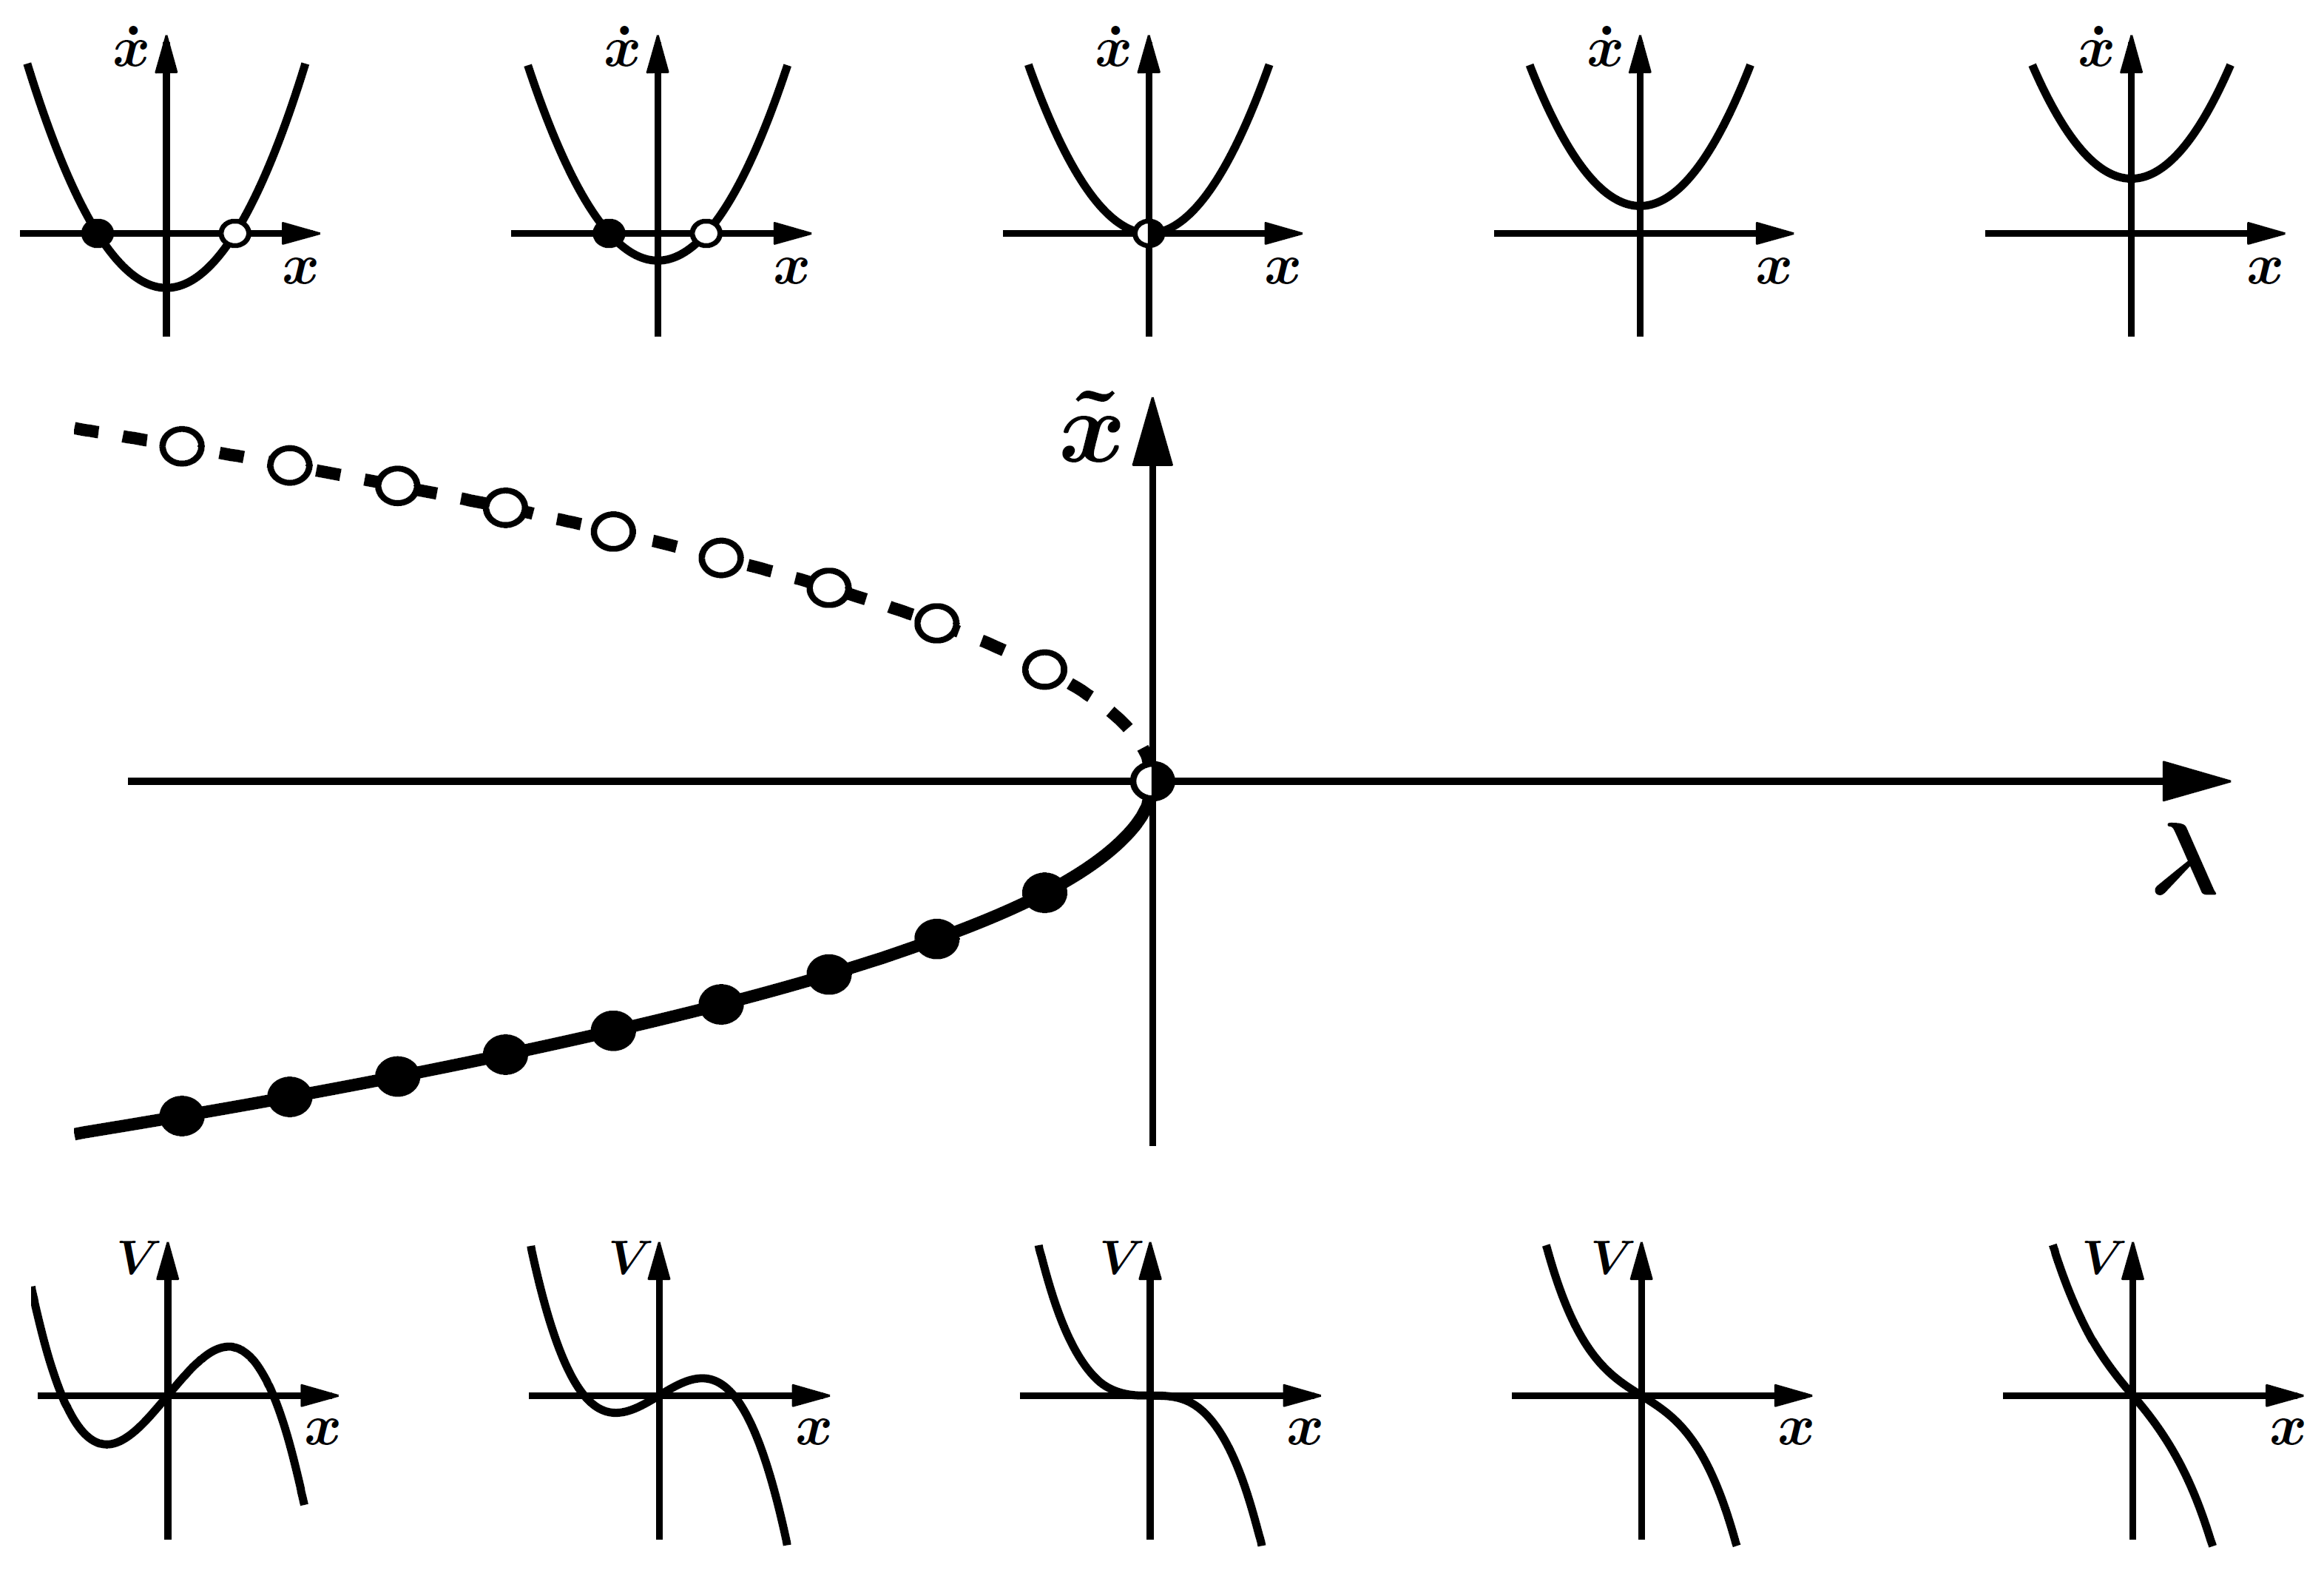
\includegraphics[width=\linewidth]{snbf.png}
    \caption{Saddle-node bifurcation.}
    \label{fig:snbf}
  \end{subfigure}
  \vline
  \begin{subfigure}{0.45\linewidth}
    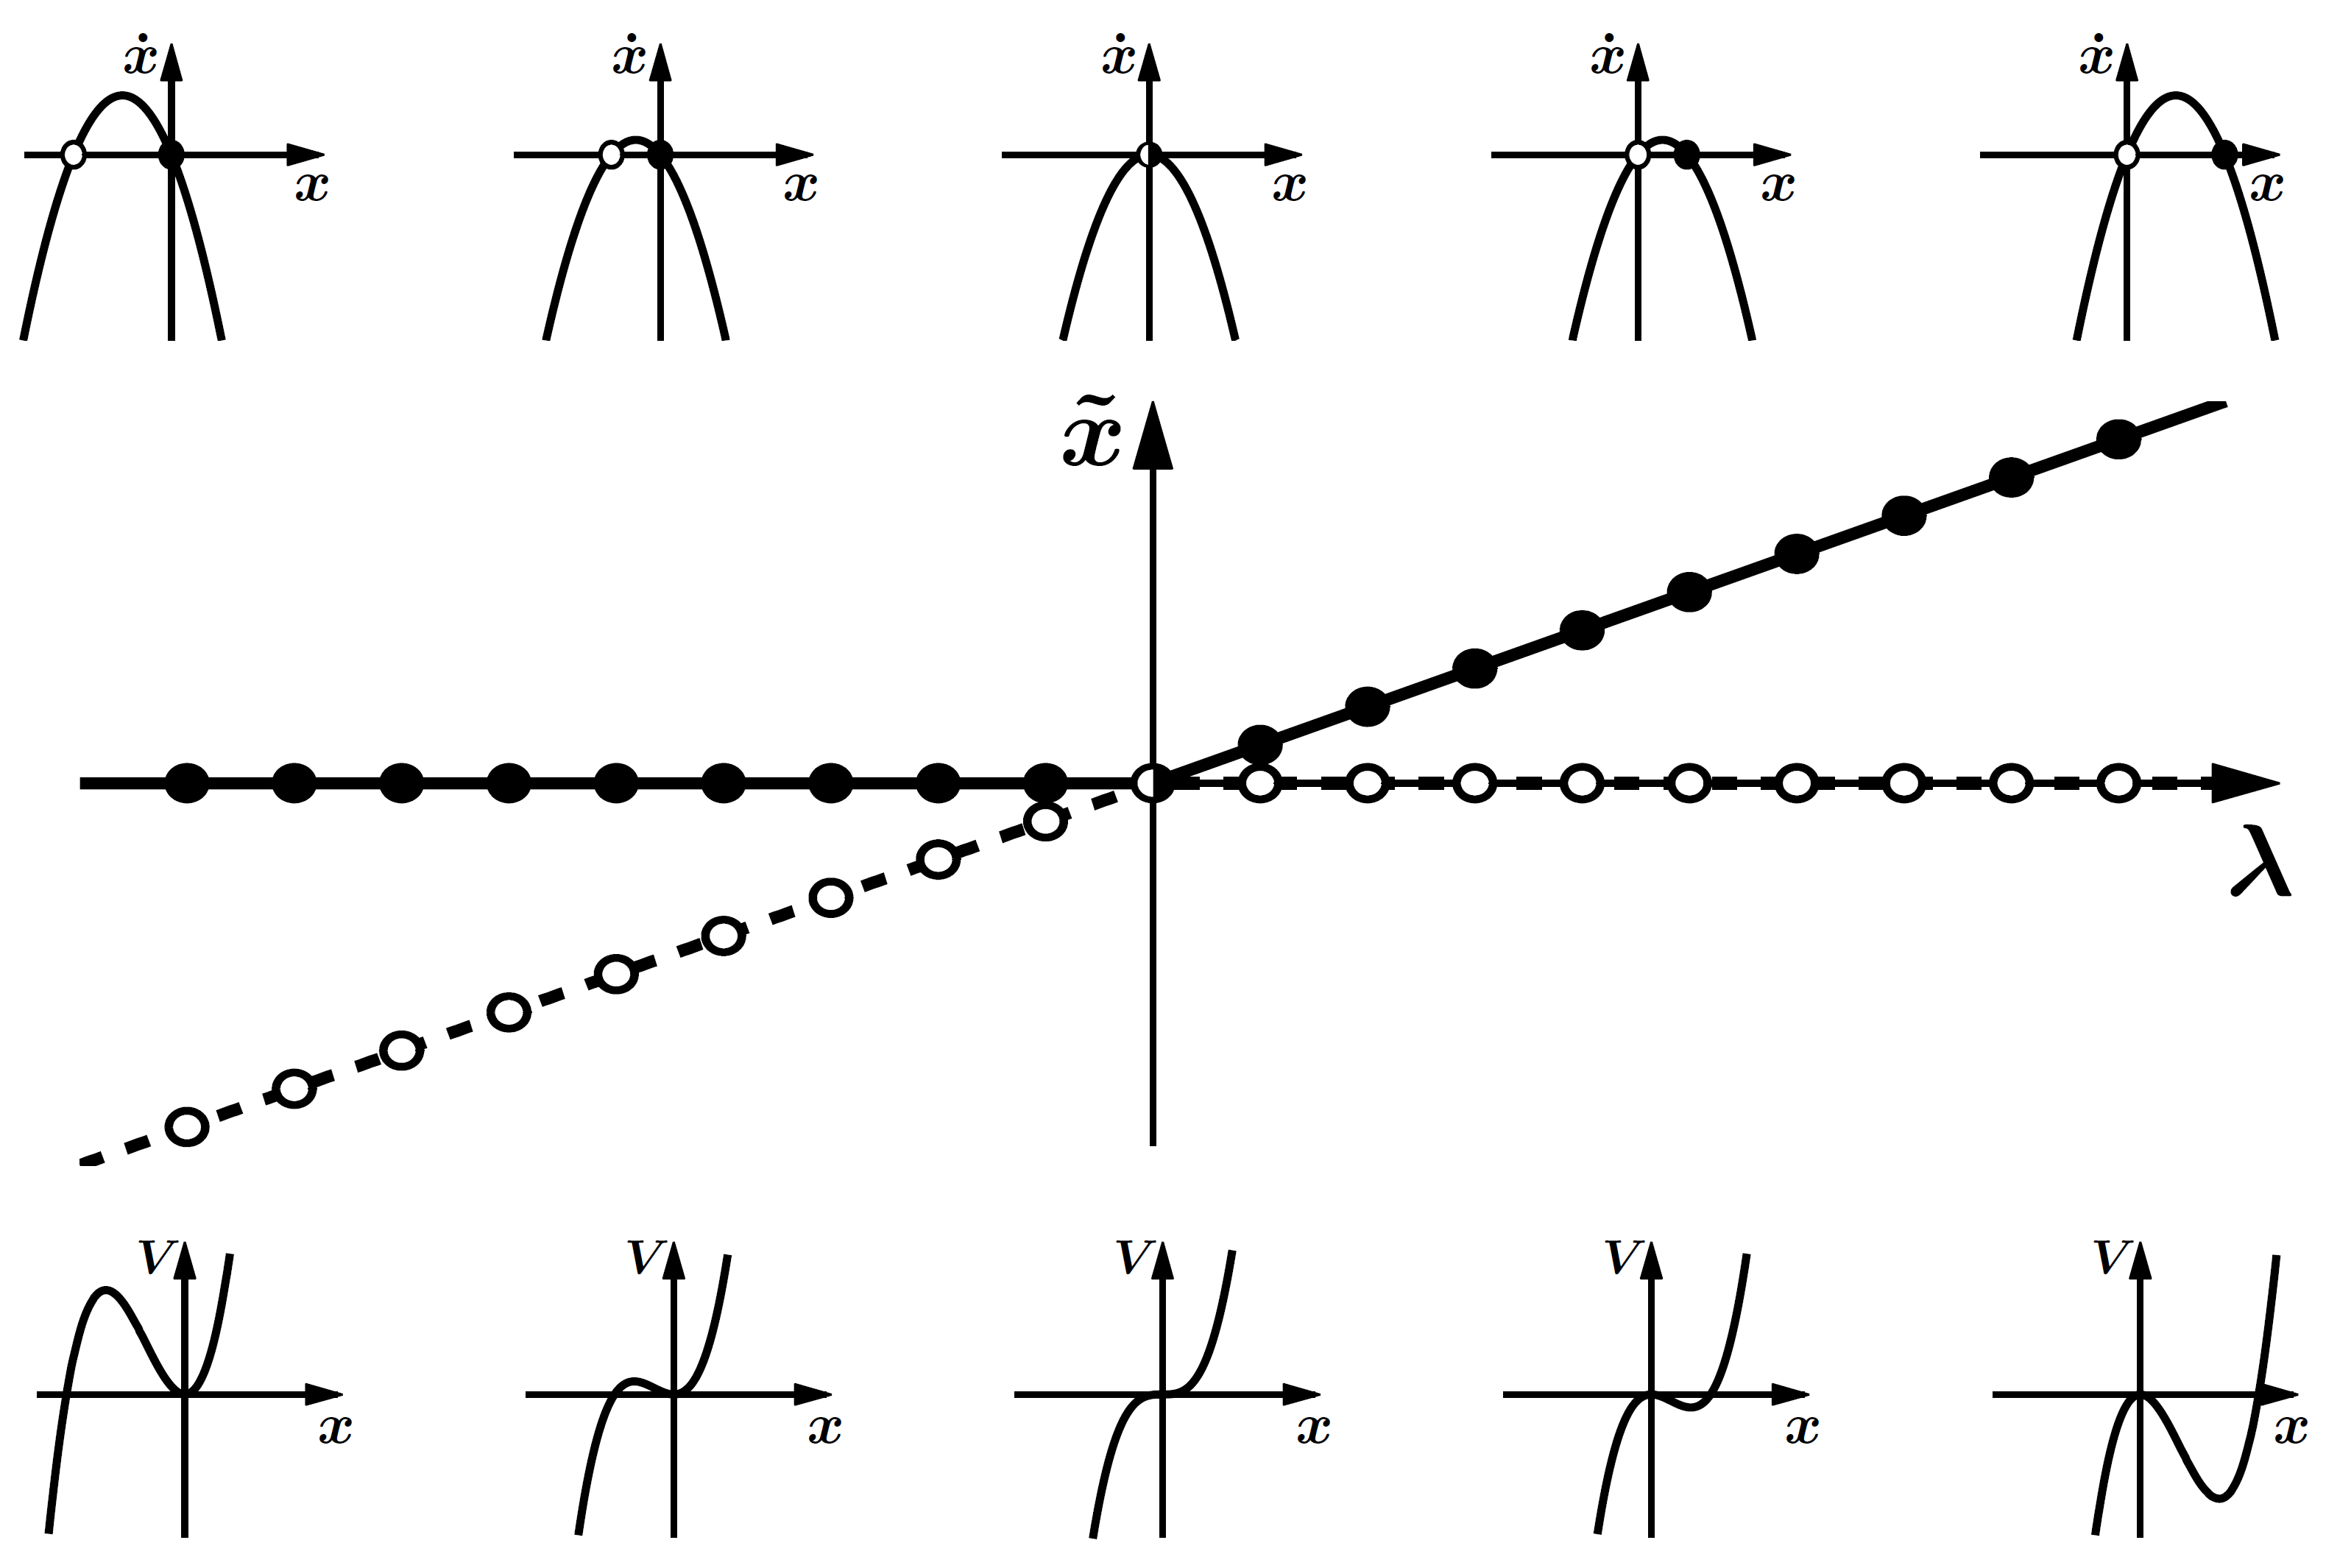
\includegraphics[width=\linewidth]{tbf.png}
    \caption{Transcritical bifurcation.}
    \label{fig:tbf}
  \end{subfigure}
  \caption{Top: phase space plots; middle: bifurcation diagram; bottom: potential functions.}
  \label{fig:stbf}
\end{figure}
\subsubsection{Transcritical Bifurcation}
The transcritical bifurcation is given by
\begin{equation}{\label{eq:tbf}}
  \dot{x}=\lambda x-x^2 \quad \rightarrow \quad \tilde{x}_1=0, \tilde{x}_2=\lambda
\end{equation}
The system has a stable and an unstable fixed point for all values except for $\lambda=0$ (Figure (\ref{fig:tbf})).
The bifurcation diagram consists of two straight lines, one given by $\tilde{x}=0$ and one with a slope of one.
When these lines intersect at the origin the fixed points they \emph{exchange stability}.
\subsubsection{Supercritical Pitchfork Bifurcation}{\label{sec:spcpbf}}
The supercritical pitchfork bifurcation is visualized in Figure (\ref{fig:spbf}) and prototypically given by
\begin{equation}{\label{eq:spbf}}
  \dot{x}=\lambda x- x^3 \quad \rightarrow \quad \tilde{x}_1=0, \tilde{x}_{2,3}=\pm\sqrt{\lambda}
\end{equation}
A single stable fixed point at the origin becomes unstable and a pair of stable fixed points appears symmetrically around $\tilde{x}=0$.
In terms of symmetry this system has an interesting property: the equation(\ref{eq:spbf}) is invariant if we substitute $x$ by $-x$.
All phase plots have a point symmetry with respect to the origin and the plots of the potential have a mirror symmetry with respect to the vertical axis (Figure (\ref{fig:spbf})).
When $\lambda>0$, the slightest perturbation will move the ball to the left or right where the slope is finite and it will settle down in one of the new minima as in Figure (\ref{fig:spbf})(bottom right).
This phenomenon is called \emph{spontaneous symmetry breaking}.
\begin{figure}[h!]
  \centering
  \begin{subfigure}{0.45\linewidth}
    \centering
    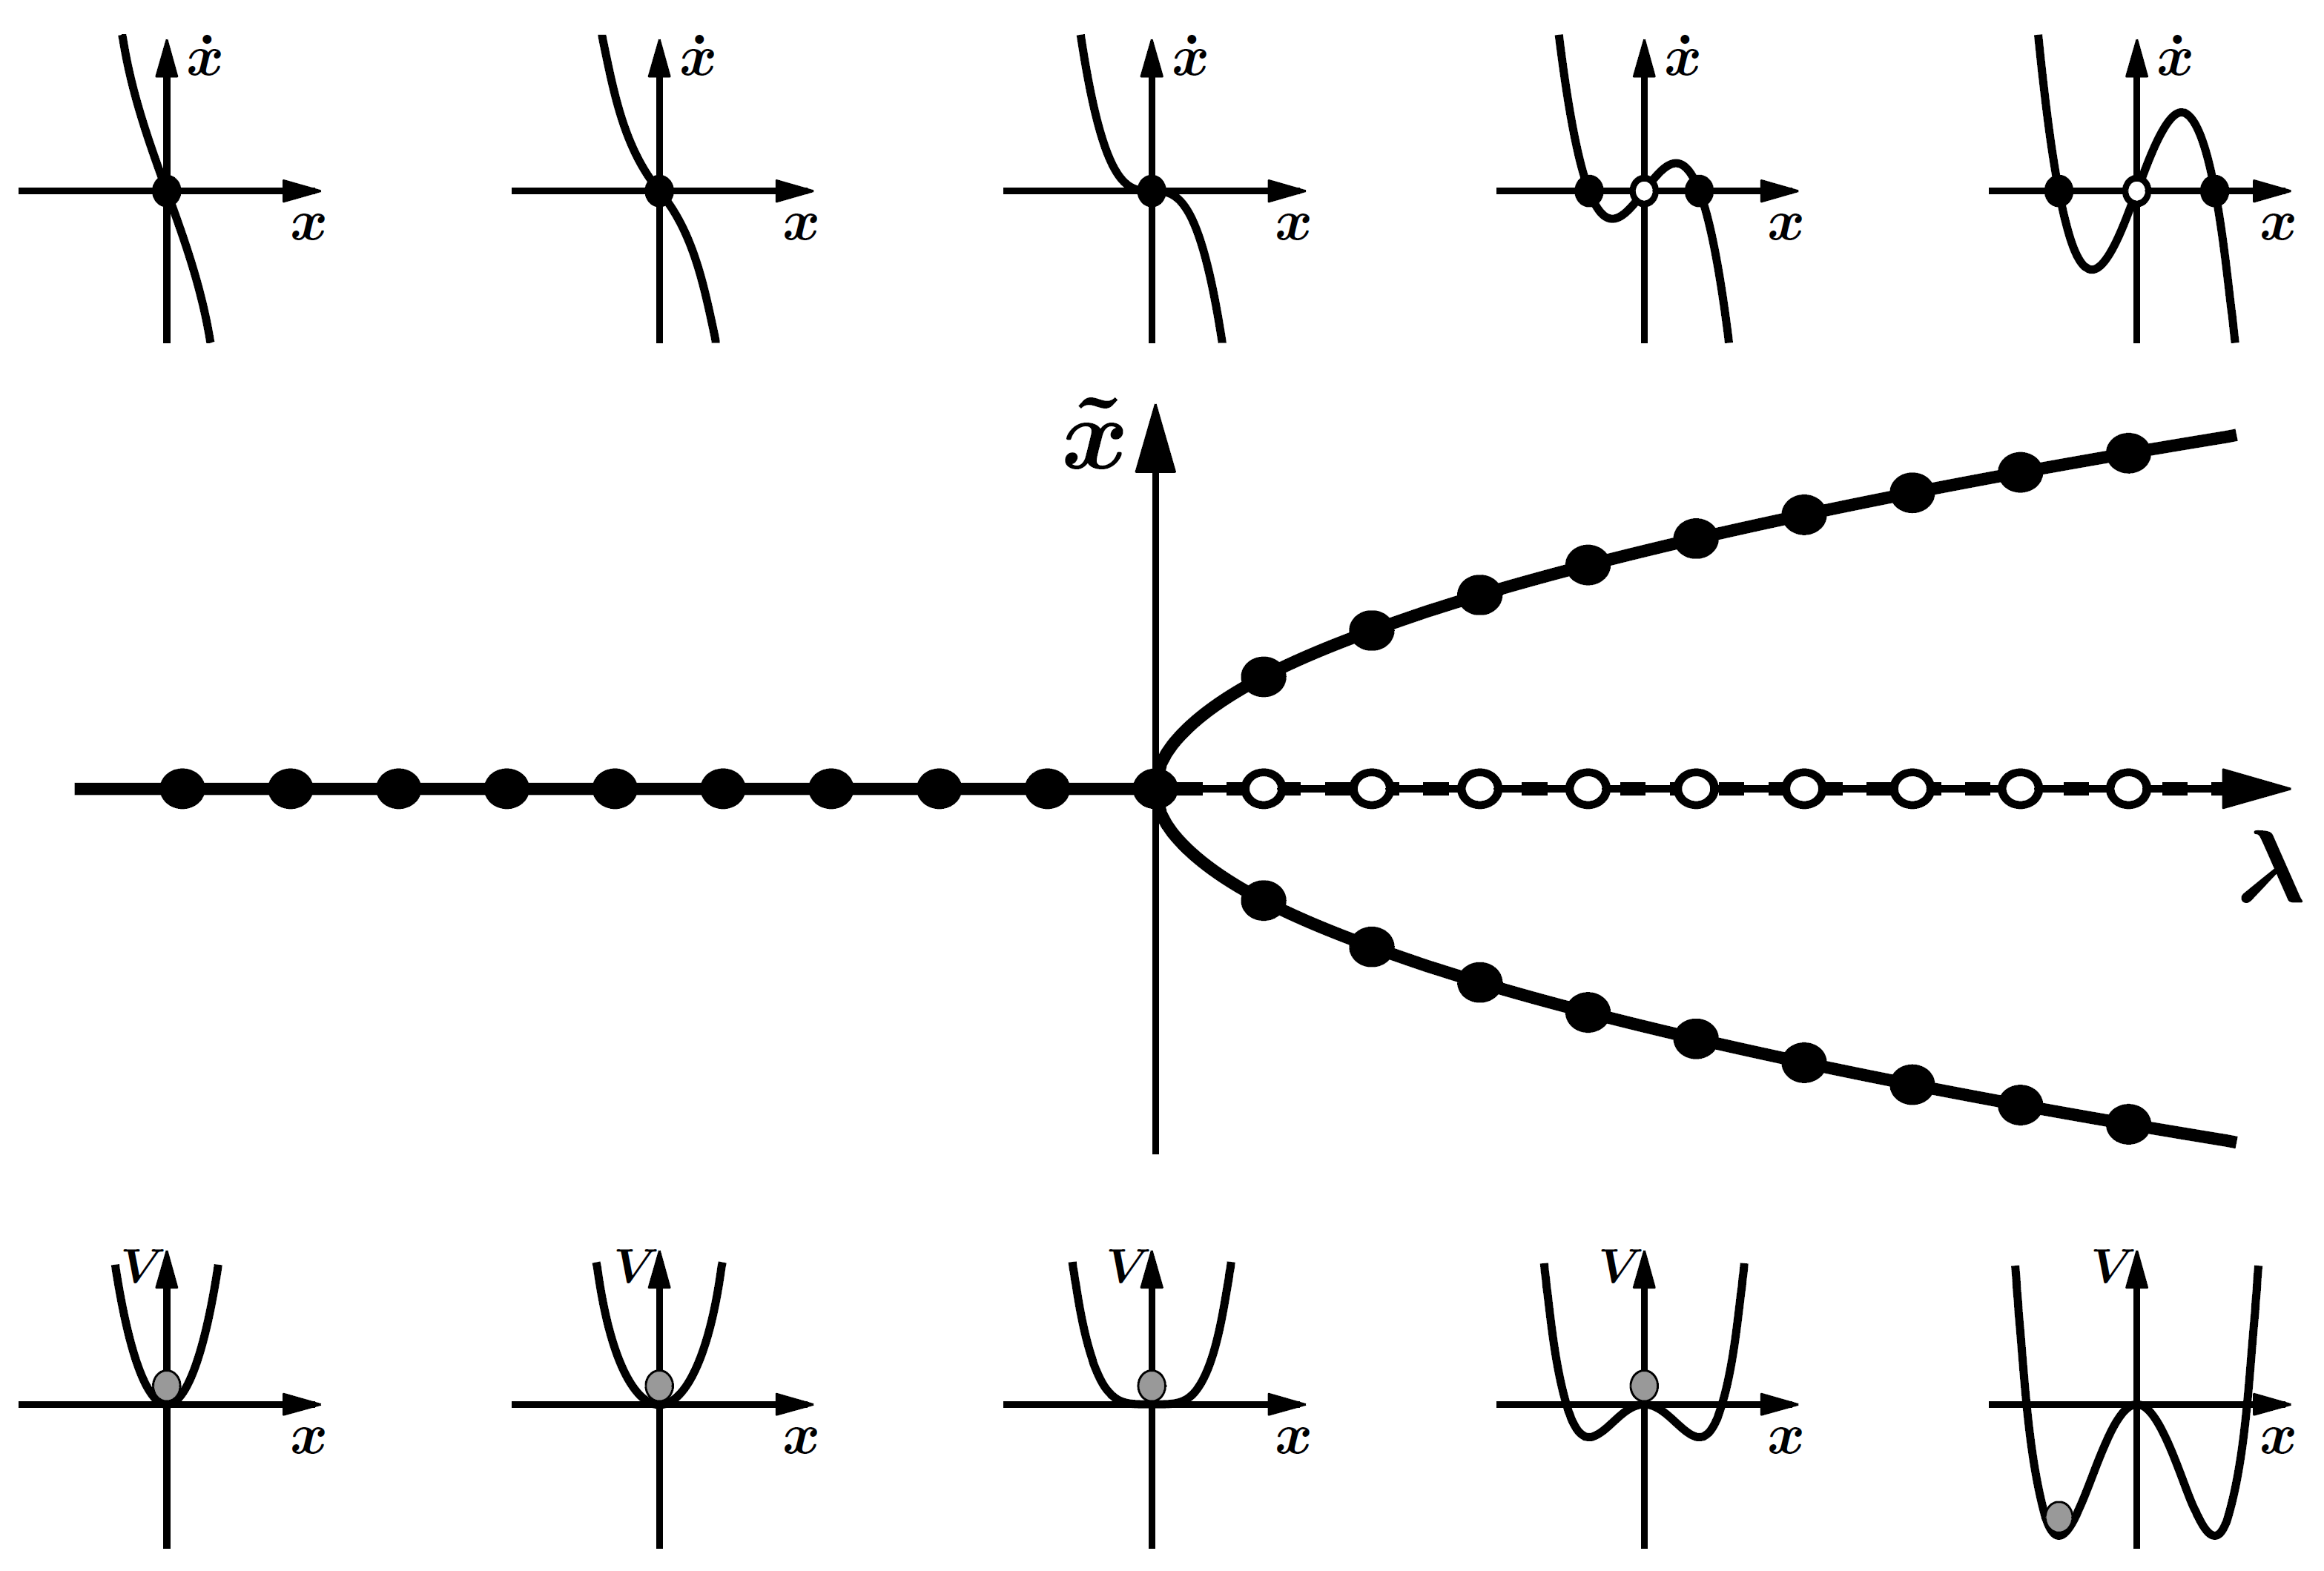
\includegraphics[width=\linewidth]{spbf.png}
    \caption{Supercritical Pitchfork bifurcation.}
    \label{fig:spbf}
  \end{subfigure}
  \vline
  \begin{subfigure}{0.45\linewidth}
    \centering
    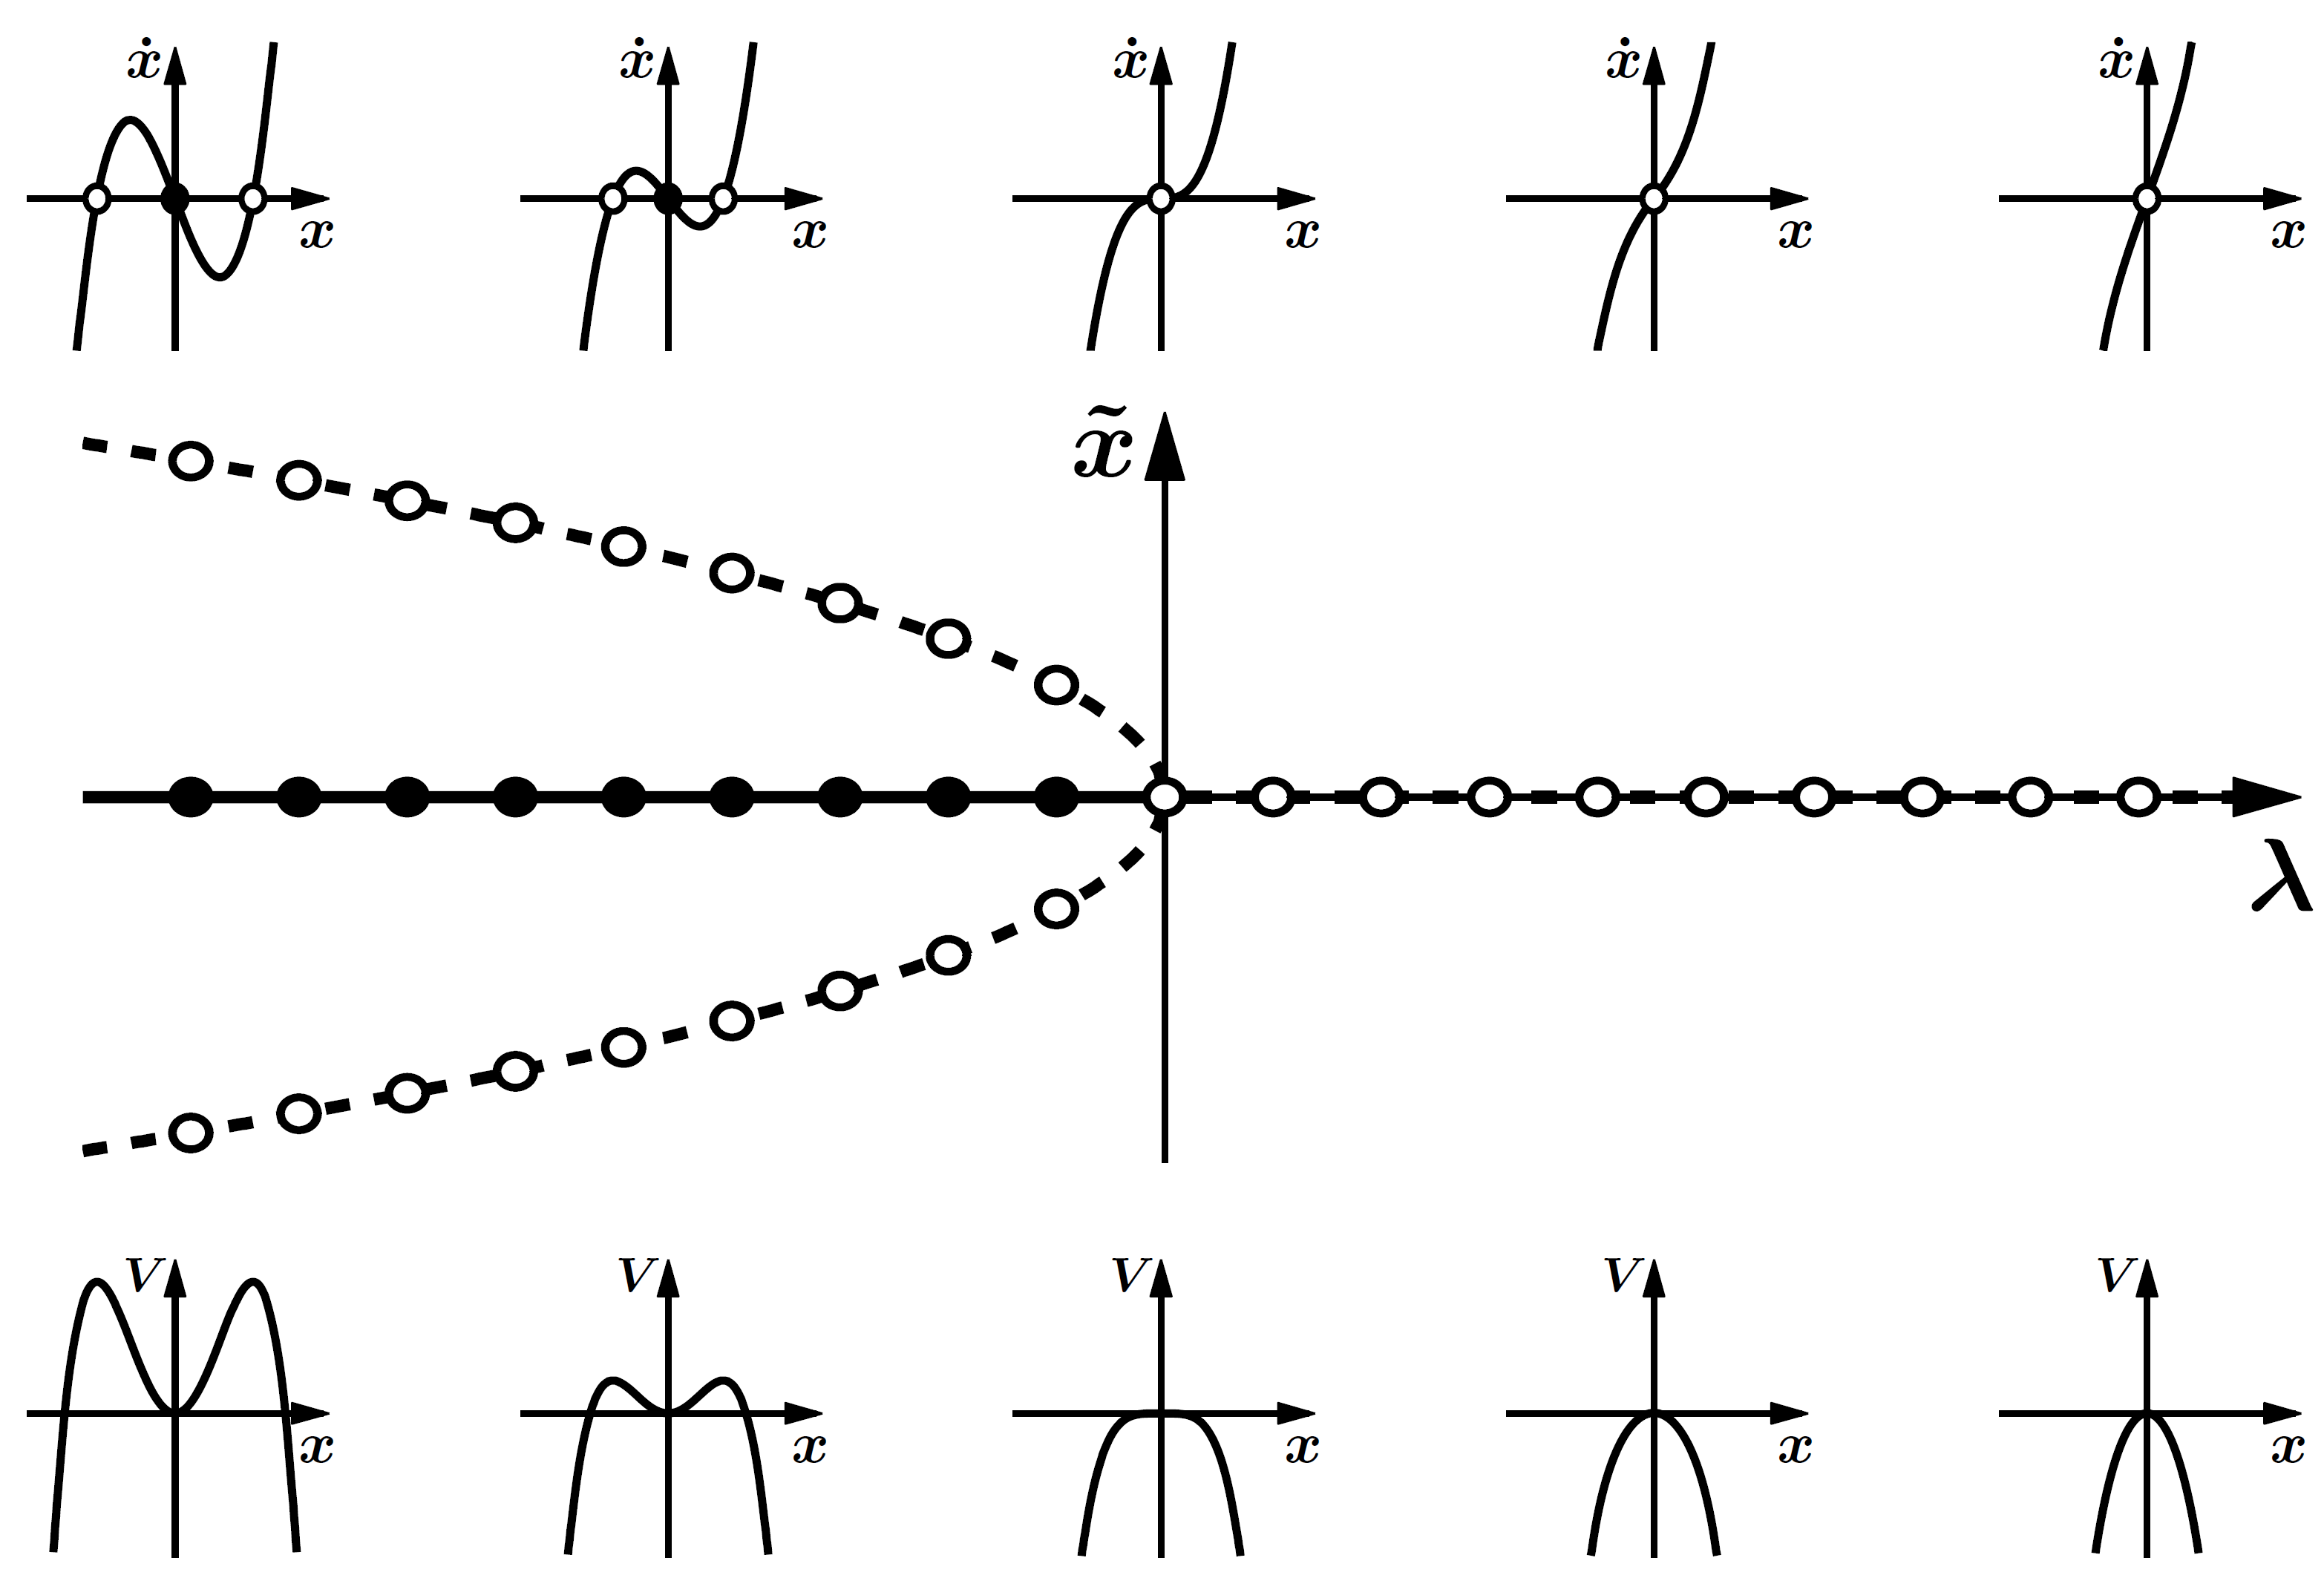
\includegraphics[width=\linewidth]{sbbf.png}
    \caption{Subcritical Pitchfork bifurcation.}
    \label{fig:sbbf}
  \end{subfigure}
  \caption{Top: phase space plots; middle: bifurcation diagram; bottom: potential functions.}
  \label{fig:sbf}
\end{figure}
\subsubsection{Subcritical Pitchfork Bifurcation}
The equation governing the subcritical pitchfork bifurcation is given by
\begin{equation}\label{eq:sbbf}
  \dot{x}=\lambda x+ x^3 \quad \rightarrow \quad \tilde{x}_1=0, \tilde{x}_{2,3}=\pm\sqrt{-\lambda}
\end{equation}
As in the supercritical case, the origin is stable for negative values of $\lambda$ and becomes unstable when the parameter exceeds $\lambda =0$ (Figure (\ref{fig:sbbf})).
Two additional fixed points exist for negative parameter values of $\lambda$ at $\tilde{x}=\pm\sqrt{-\lambda}$ and they are both repellers.
\begin{theorem}[\textbf{Bifurcations}]
  Suppose the system $\dot{x}(t)=f(x,\lambda), x,\lambda\in\mathbb{R}$ has an equilibrium point $x=x_0$ at $\lambda=\lambda_0$ satisfying the conditions
  \begin{equation}
    f(x_0,\lambda_0)=0\qquad\frac{\partial f}{\partial x}(x_0,\lambda_0)=0
  \end{equation}
  \begin{itemize}
    \item
    \begin{equation}
      \frac{\partial f}{\partial \lambda}(x_0,\lambda_0)\neq0\quad\frac{\partial^2 f}{\partial x^2}(x_0,\lambda_0)\neq0
    \end{equation}
    The system has a saddle-node bifurcation at $(x_0,\lambda_0)$.
    \item
    \begin{equation}
      \frac{\partial f}{\partial \lambda}(x_0,\lambda_0)=0\quad\frac{\partial^2 f}{\partial x^2}(x_0,\lambda_0)\neq0\quad\frac{\partial^2f}{\partial x\partial y}(x_0,\lambda_0)\neq0
    \end{equation}
    The system has a transcritical bifurcation at $(x_0,\lambda_0)$.
    \item
    \begin{equation}
      \frac{\partial f}{\partial \lambda}(x_0,\lambda_0)=0\quad\frac{\partial^2 f}{\partial x^2}(x_0,\lambda_0)=0\quad\frac{\partial^2f}{\partial x\partial y}(x_0,\lambda_0)\neq0\quad\quad\frac{\partial^3f}{\partial x^3}(x_0,\lambda_0)\neq0
    \end{equation}
    The system has a pitchfork bifurcation at $(x_0,\lambda_0)$.
  \end{itemize}
\end{theorem}
\subsection{Bifurcations and Hysteresis}
In equation, 
\begin{equation}
  \dot{x}=\lambda+x-x^3
\end{equation}
Depending on whether the parameter is increased from large negative or decreased from large positive values the switch occurs at $\lambda=\lambda_c$ or $\lambda=-\lambda_c$, respectively.
It consists of two saddle-node bifurcations indicated by the dotted rectangles in Figure (\ref{fig:bfwh1}).
\begin{figure}[h!]
  \centering
  \begin{subfigure}{0.45\linewidth}
    \raggedleft
    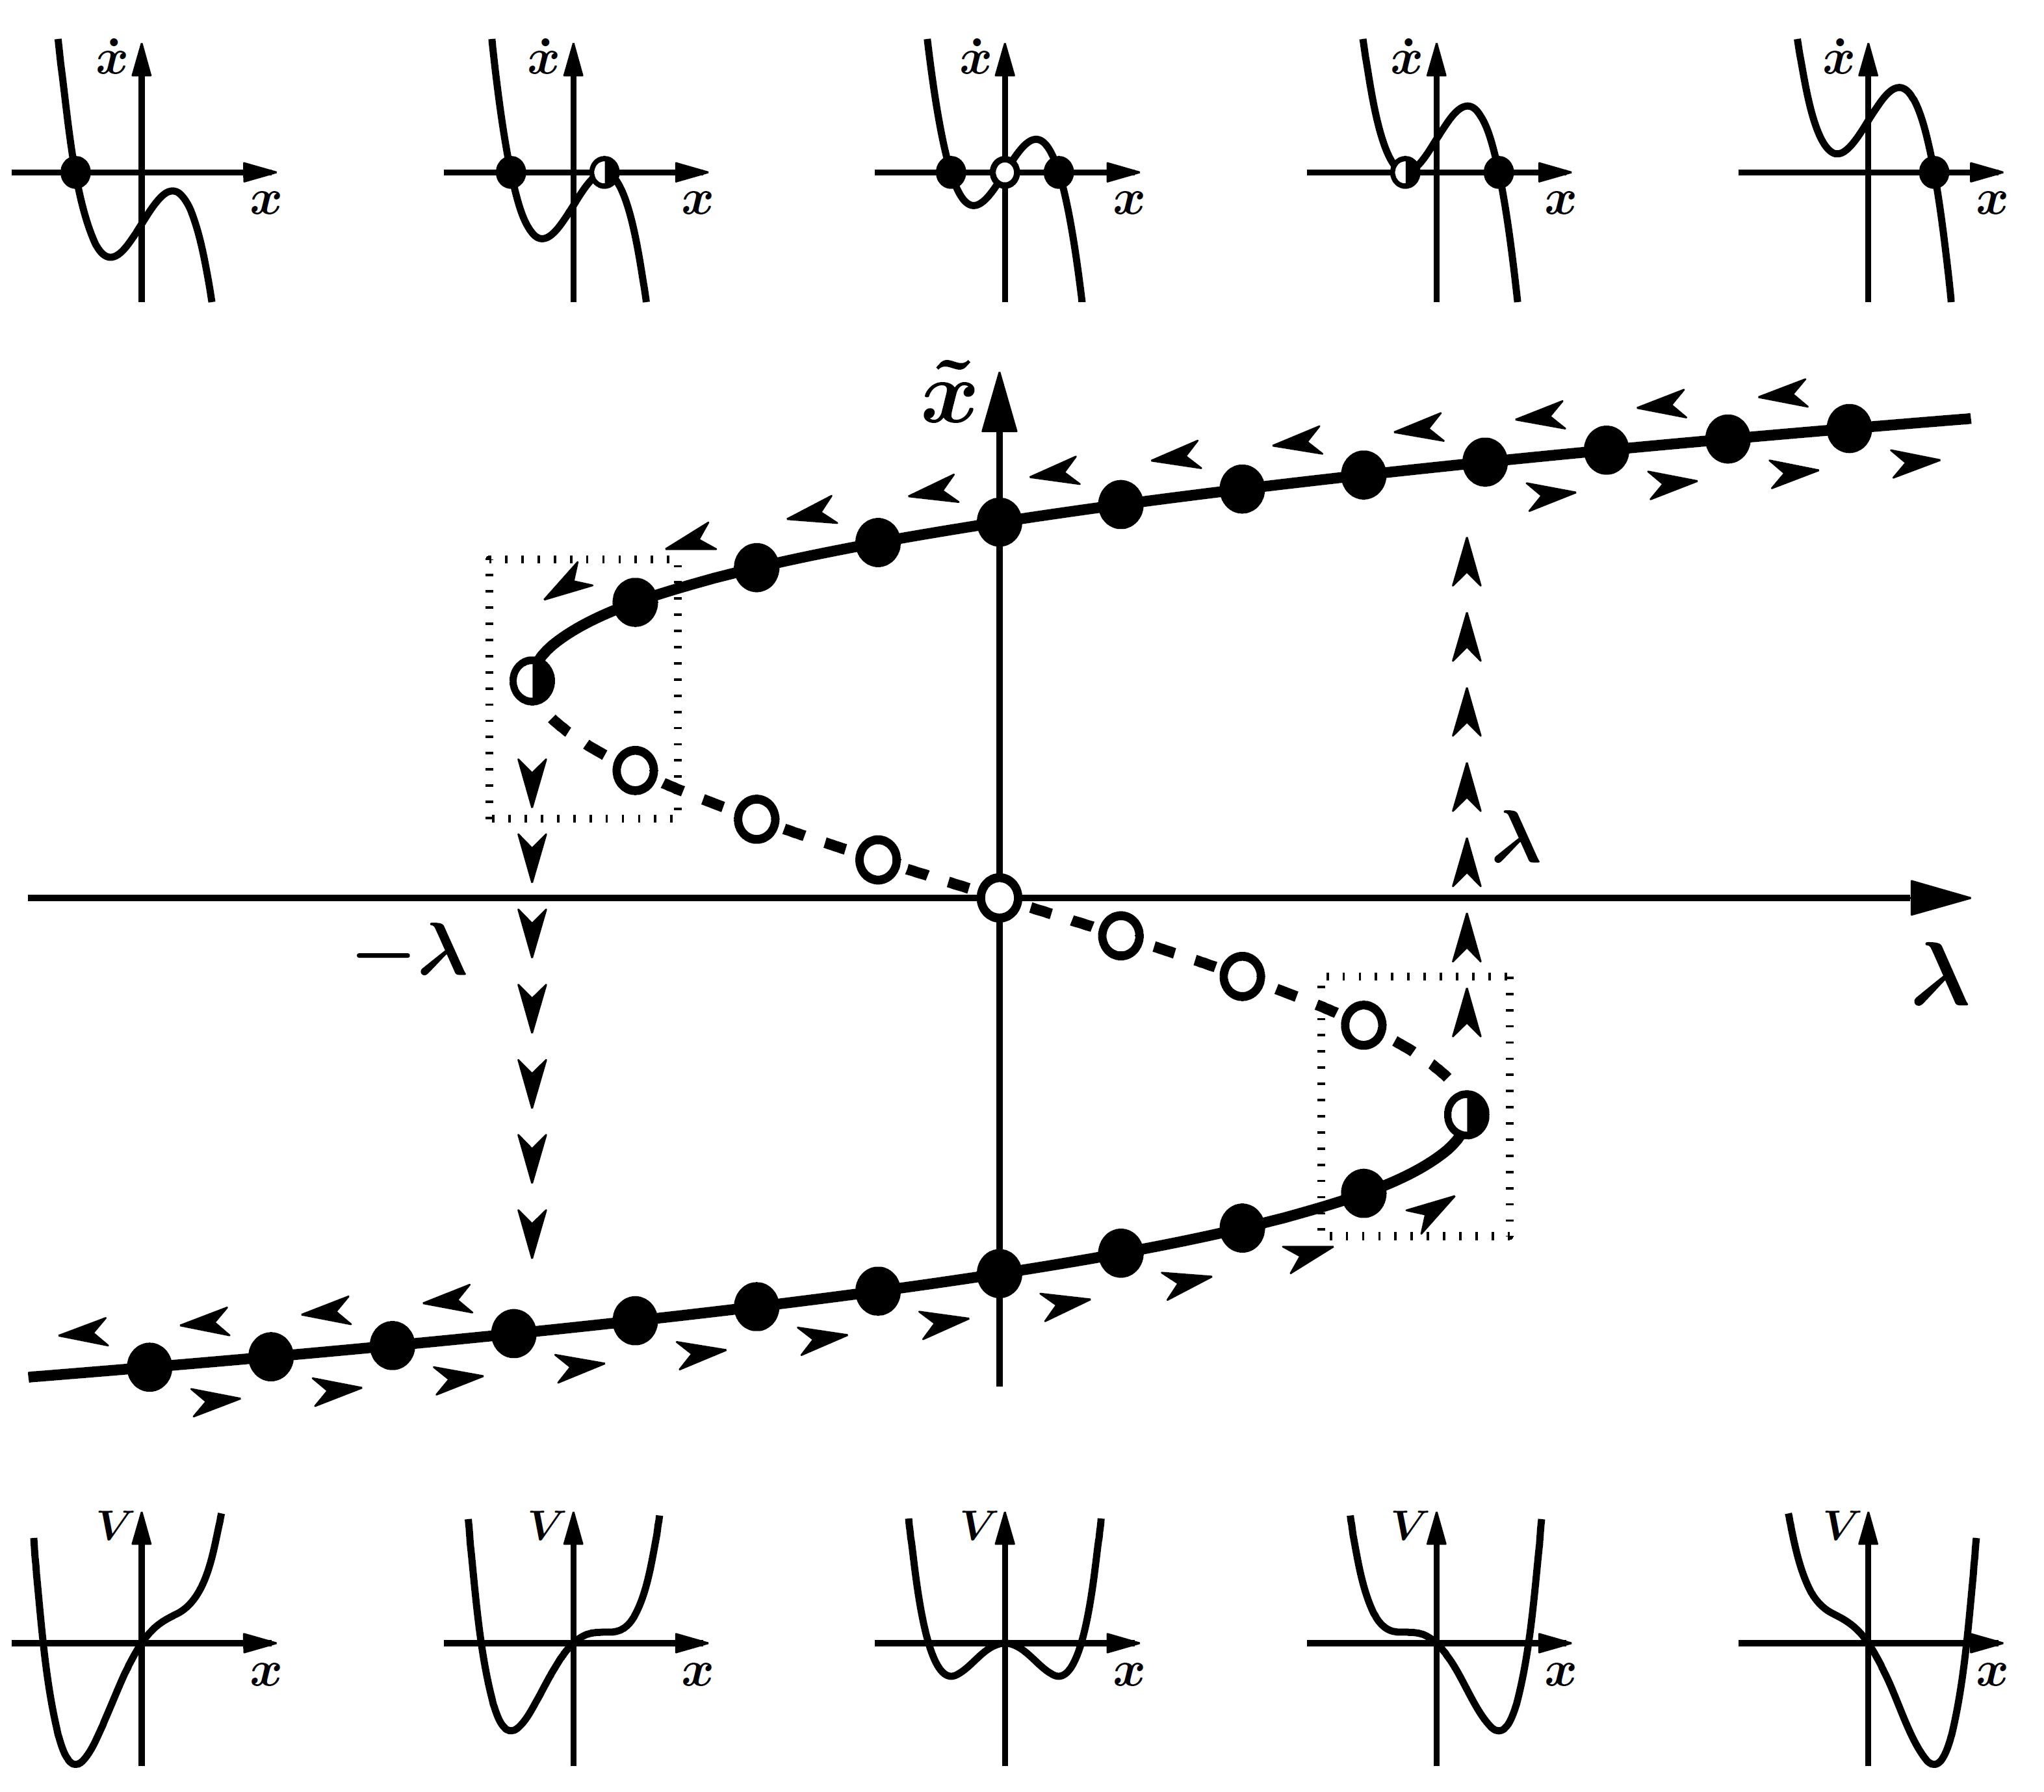
\includegraphics[width=\linewidth]{bfwh1.png}
    \caption{$\dot{x}=\lambda+x-x^3$}
    \label{fig:bfwh1}
  \end{subfigure}
  \vline
  \begin{subfigure}{0.45\linewidth}
    \raggedright
    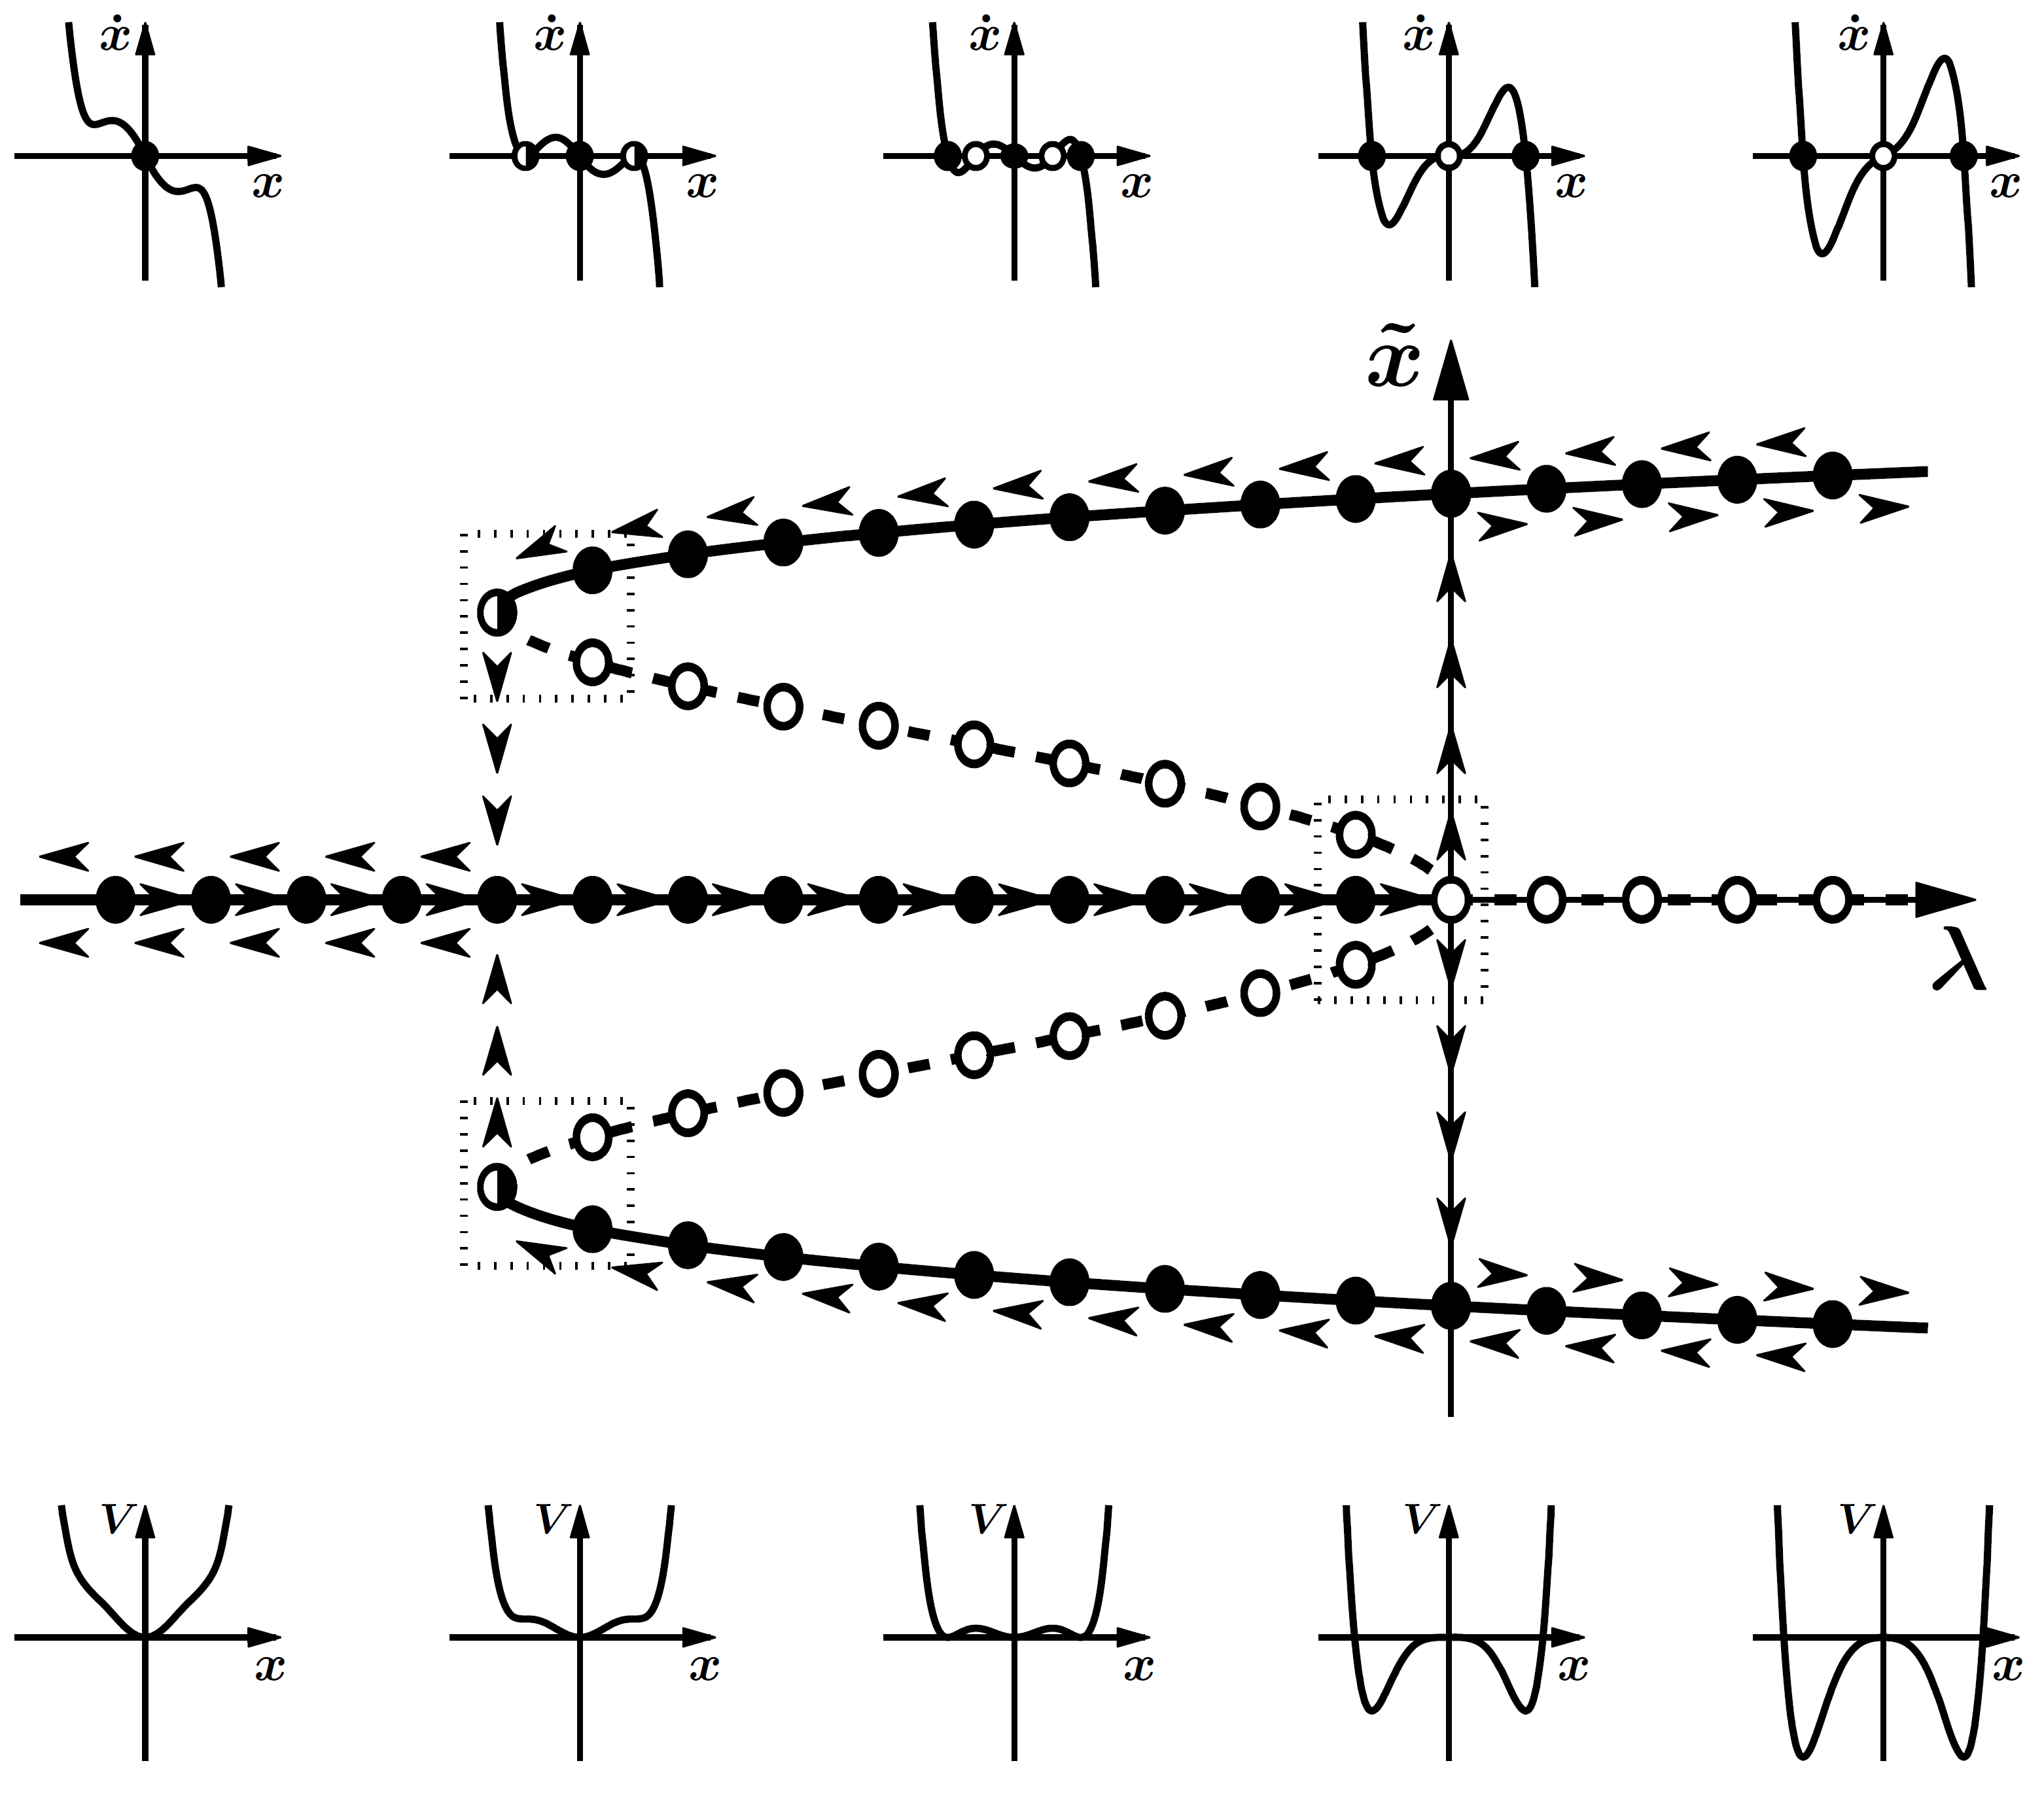
\includegraphics[width=\linewidth]{bfwh2.png}
    \caption{$\dot{x}=\lambda x+x^3-x^5$}
    \label{fig:bfwh2}
  \end{subfigure}
  \caption{Systems showing hysteresis.}
  \label{fig:bfwh}
\end{figure}
\paragraph{Globally Stable Subcritical Pitchfork Bifurcation}
In equation, 
\begin{equation}
\dot{x}=\lambda x+x^3-x^5
\end{equation}
A globally stable version of the subcritical pitchfork bifurcation.
The diagram contains three basic bifurcations indicated by the dotted rectangles in Figure (\ref{fig:bfwh2}).
Beside the subcritical pitchfork bifurcation at the origin there are two saddle-node bifurcations at locations $\lambda=-\frac{1}{4}$, $\tilde{x}=\pm\frac{1}{2}\sqrt{2 }$ in the $\lambda\tilde{x}-$plane.